
%(BEGIN_QUESTION)
% Copyright 2006, Tony R. Kuphaldt, released under the Creative Commons Attribution License (v 1.0)
% This means you may do almost anything with this work of mine, so long as you give me proper credit

I motsetning til lineære funksjoner har ikke grafene til ikke-lineære funksjoner konstant {\it stigningstall}. Ta for eksempel denne grafen av en ``parabel'' på formen $y = x^2$:

$$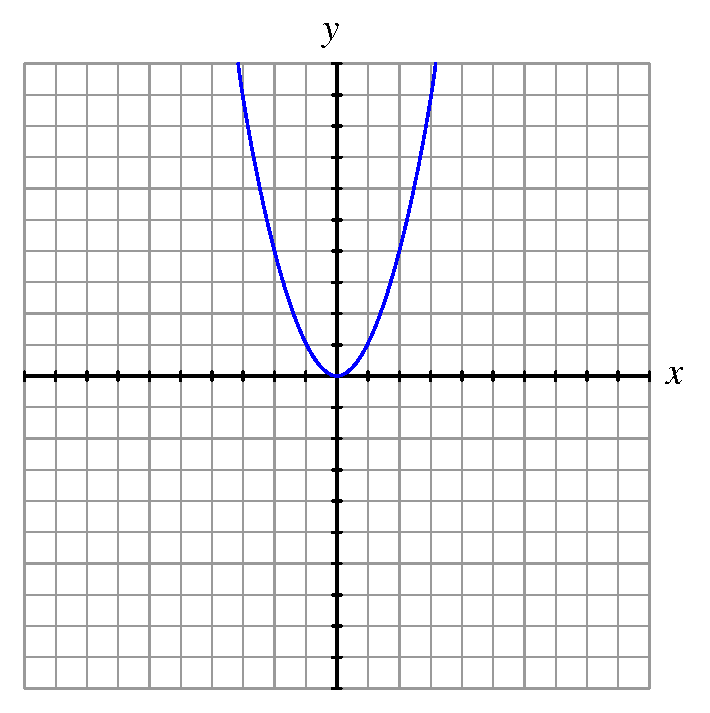
\includegraphics[width=15.5cm]{i01515x01.eps}$$

Det er vanskelig (men ikke umulig) å anslå stigningstallet til en ikke-lineær funksjon som denne i et gitt punkt, bare ved å se på grafen. Hvis jeg ba deg anslå stigningstallet til denne funksjonens graf ved $x=2$, hvordan ville du gjort det?

\underbar{file i01515}
%(END_QUESTION)





%(BEGIN_ANSWER)

En måte er å tegne en linje som så vidt berører parabelkurven i koordinatet (2,4), og anslå stigningstallet til denne linjen:

$$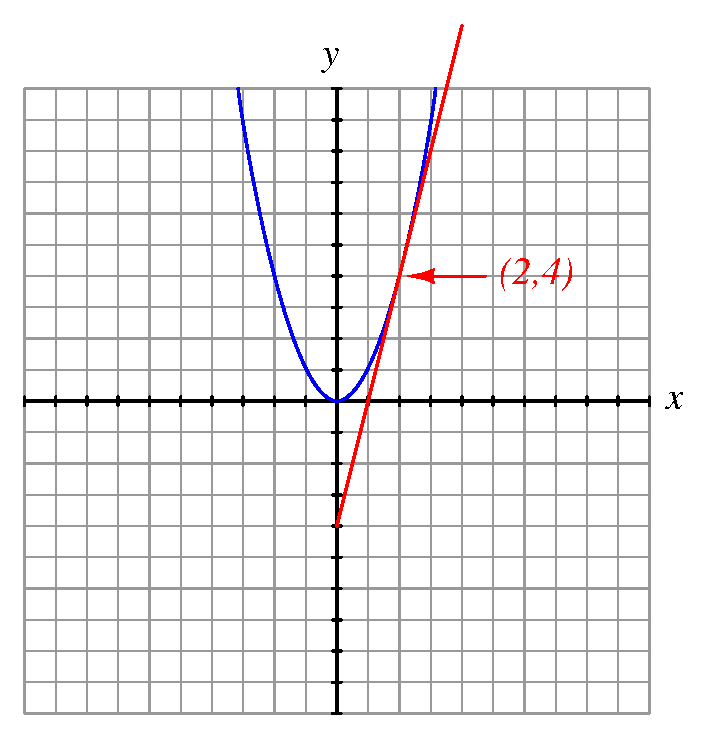
\includegraphics[width=15.5cm]{i01515x02.eps}$$

%(END_ANSWER)





%(BEGIN_NOTES)

For ordens skyld er det {\it eksakte} stigningstallet til parabelen i (2,4) lik 4.

%INDEX% Mathematics, calculus: slope of a parabola

%(END_NOTES)

